\documentclass[11pt,letterpaper]{article}

%----------------------------
%  Package Imports
%----------------------------
\usepackage[utf8]{inputenc}
\usepackage[T1]{fontenc}
\usepackage[english]{babel}

\usepackage[letterpaper,margin=25mm]{geometry}

\usepackage{tgtermes}        % TeX Gyre Termes (Times‐like). Swap to 'tgpagella' for Palatino style, etc.

% 2) Improve micro‐typography (protrusion + font expansion)
\usepackage{microtype}

% 3) Better “code” / monospaced font for any snippets
\usepackage{inconsolata}     % a clean, professional monospace


% 5) Slightly more vertical space between paragraphs (optional)
\usepackage{parskip}         % removes paragraph indentation, adds small skip

% 6) If you want “fancy” headers/footers (document title on the left, page number on the right, etc.)
\usepackage{fancyhdr}
\pagestyle{fancy}
\fancyhf{}                                  % clear all header/footer fields
\fancyhead[L]{\small NOIRLab\\ 4‐Channel ADC Module Prototype}  % left header
\fancyhead[R]{\small Version 0.1}           % right header
\fancyfoot[C]{\small \thepage}              % centered footer

% 7) For clickable, colored links in PDF
\usepackage[hidelinks]{hyperref}


% Math and symbols
\usepackage{amsmath,amssymb,mathtools}

% \usepackage{tikz}
\usepackage{circuitikz}
\usetikzlibrary{positioning, fit, calc}

% Load siunitx for SI units:
\usepackage{siunitx}
\sisetup{detect-all}

% define a general sqrt-unit macro:
\newcommand{\sqrtunit}[1]{%
  \ensuremath{%
    \sqrt{\text{\si{#1}}}%
  }%
}

% better tables
\usepackage{booktabs}

% Figures and captions
\usepackage{graphicx}
\usepackage{caption}
\usepackage{subcaption}

% Hyperlinks and cross-referencing
\usepackage[hidelinks]{hyperref}

% Page geometry
% \usepackage[a4paper,margin=2.5cm]{geometry}

% Bibliography (if you cite datasheets or papers)
\usepackage{cite}

%----------------------------
%  Document Begins
%----------------------------
\begin{document}

% Title page
\title{4-Channel ADC Module Prototype\\Module Description and Analysis}
\author{Braulio Cancino Vera \\ National Optical-Infrared Astronomy Research Laboratory (NOIRLab)}
\date{Version 0.1}
\maketitle

% Table of Contents (clickable)
\tableofcontents
\clearpage

% Include each section in order
\section{Introduction}
\label{sec:intro}

This document describes the schematic and functional operation of a 4-channel ADC module prototype, designed in KiCad 9. The module is one building block in a scalable detector-controller system: each board contains its own processor and plugs into a minimal backplane that provides:
\begin{itemize}
  \item A single \SI{12}{\volt} power rail.
  \item A \SI{10}{\mega\hertz} synchronization clock for the DC-DC converters and the detector sequencer
  \item A start signal indicating the beginning of an acquisition cycle.
  \item An emergency-stop line to flag a fault condition.
\end{itemize}
Each board also has its own Gigabit Ethernet port—for configuration, telemetry, and streaming video data

\autoref{fig:pcb_top} and \autoref{fig:pcb_bottom} show the PCB implementation of the 4-channel ADC prototype board with

\begin{multicols}{2}
  \begin{enumerate}
    \item Digital \SI{3.3}{\volt} DC-DC Converter.
    \item Backplane Connector.
    \item Analog \SI{-15.5}{\volt} DC-DC Converter.
    \item RJ45 Ethernet Connector.
    \item Zynq-Soc Module Mode Switch.
    \item Voltage Translator IC.
    \item Analog \SI{5.5}{\volt} DC-DC Converter.
    \item Analog \SI{15.5}{\volt} DC-DC Converter.
    \item FTDI USB-C Interface.
    \item Zynq-Soc Module.
    \item Zynq-Soc Reset Button.
    \item Digital \SI{2.5}{\volt} LDO.
    \item 4 Channel Video Front-End and ADC.
    \item Analog \SI{5}{\volt} LDO.
    \item Analog \SI{2.5}{\volt} LDO.
    \item Analog \SI{4.2}{\volt} LDO.
    \item Analog \SI{15}{\volt} LDO.
    \item Analog \SI{-15}{\volt} LDO.
    \item Video Input Connector.
    \item \SI{12}{\volt} Power Input Protection.
    \item Clock Generator.
    \item EEPROM.
  \end{enumerate}
\end{multicols}

\begin{figure}[!ht]
  \centering
   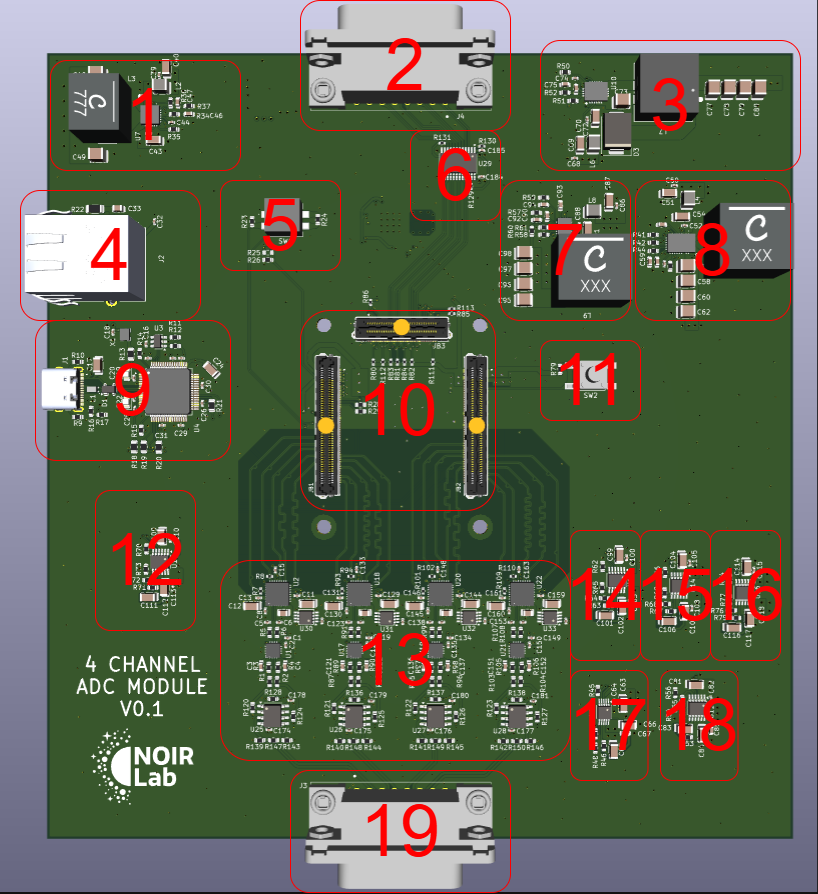
\includegraphics[width=0.8\linewidth]{sections/introduction/top_number.png}
  \caption{Top View of the 16.2 cm x 17.1 cm, six-layer PCB with impedance control, 4-channel ADC prototype board.}
  \label{fig:pcb_top}
\end{figure}

\begin{figure}[!ht]
  \centering
   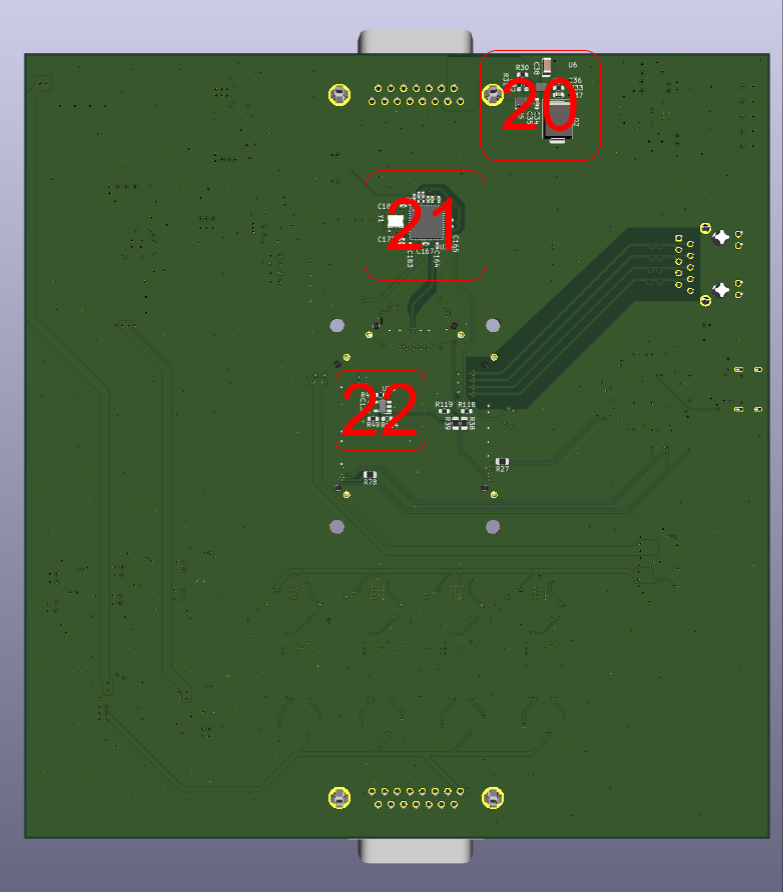
\includegraphics[width=0.8\linewidth]{sections/introduction/bottom_number.png}
  \caption{Bottom View of the 16.2 cm x 17.1 cm, six-layer PCB with impedance control, 4-channel ADC prototype board.}
  \label{fig:pcb_bottom}
\end{figure}

In \autoref{fig:pcb_top}, most of the digital circuitry is clustered on the left side (from top view). Along the top edge you'll find the backplane connector and the DC-DC converters; along the bottom edge are the low-noise LDOs, the four ADC channels with their analog front end, and the input connector.

Immediately beside the top backplane connector, a jitter-attenuator clock generator takes the 10 MHz sync clock from the backplane and delivers a low-jitter reference to the Zynq SoC for the detector sequencer and DC-DC synchronization. A small I²C EEPROM stores the board's type and revision information.

At the center of the board sits a Trenz TE0720-04-62I33MA Zynq SoC-Module, which integrates an AMD Zynq™ 7020-2I, 1 GB of DDR3L RAM, and 8 GB of eMMC flash.

On the left digital side, a Gigabit-Ethernet RJ45 port interfaces with the Zynq SoC for configuration, telemetry, and streaming video data from the ADCs. An FTDI USB-C interface provides direct programming of the Zynq (without a separate JTAG adapter) and supplies a UART console link
\section{Power}
\label{sec:power}

\subsection{\SI{12}{\volt} Input Protection}

As \SI{12}{\volt} input protection we use a TPS259480AYWPR Texas Instruments eFuse that features:

To safeguard the \SI{12}{\volt} supply, we employ a Texas Instruments TPS259480A e-Fuse, which integrates back-to-back MOSFETs and offers the following features:

\begin{itemize}
    \item Integrated back-to-back FETs with low ON resistance $R_\mathrm{ON}=\SI{12.2}{\milli\ohm}$.
    \item Ideal diode operation with true reverse current blocking.
    \item Fast overload protection.
    \item Overcurrent protection with load current monitor.
    \item Fast-trip response for short circuit protection.
    \item Adjustable output slew rate.
\end{itemize}

Upstream of the e-Fuse, a TI TVS1800DRV \SI{18}{\volt} flat-clamp transient-voltage suppressor absorbs voltage spikes and surges on the \SI{12}{\volt} line. Downstream, a B520C \SI{20}{\volt}, \SI{5}{\ampere} Schottky diode provides secondary overvoltage protection at the e-Fuse output. \autoref{fig:power_12vin} illustrate the complete \SI{12}{\volt} input protection circuit.

\begin{figure}[ht]
  \centering
  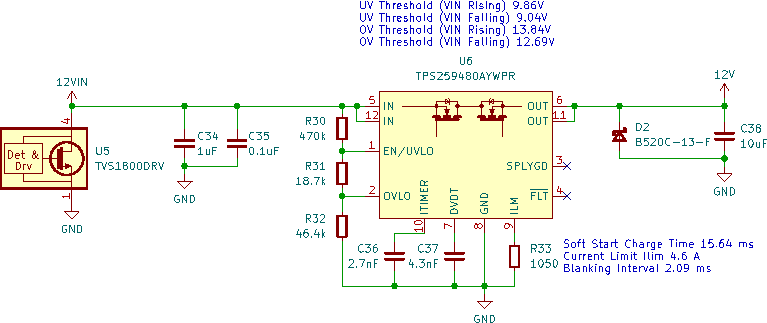
\includegraphics[width=0.8\linewidth]{sections/power/fig_12vin.pdf}
  \caption{\SI{12}{\volt} Input Protection Circuit}
  \label{fig:power_12vin}
\end{figure}


\subsection{Digital \SI{3.3}{\volt} (3V3D)}

Digital \SI{3.3}{\volt} serves as the primary supply for the Zynq SoC and feeds the \SI{2.5}{\volt} digital LDO used by the ADC. We selected the Analog Devices LT8642S synchronous step-down converter, which provides:
\begin{itemize}
    \item Ultra low EMI emissions (Silent Switcher 2 Architecture).
    \item High efficiency: up to 95\% efficiency at \SI{2}{\mega\hertz}, \SI{12}{\volt} input and \SI{3.3}{\volt} output.
    \item Up to \SI{10}{\ampere} output current.
    \item External compensation.
\end{itemize}

The LT8642S is configured to operate at \SI{2}{\mega\hertz} (see \autoref{fig:power_3v3d}). A Coilcraft XGL1010-801 shielded inductor (\SI{0.8}{\micro\henry}, \SI{0.88}{\milli\ohm} DCR) minimizes losses. Upstream of the converter input, a $\pi$ LC filter suppresses input noise. Power-Good output (\texttt{3V3D\_PG}) and the SYNC pin (\texttt{3V3D\_SYNC}) are both tied back to the Zynq SoC for voltage monitoring and clock synchronization. See LTSpice and LTPoweCAD simulation files for transient and frequency compensation design.

\begin{figure}[ht]
  \centering
  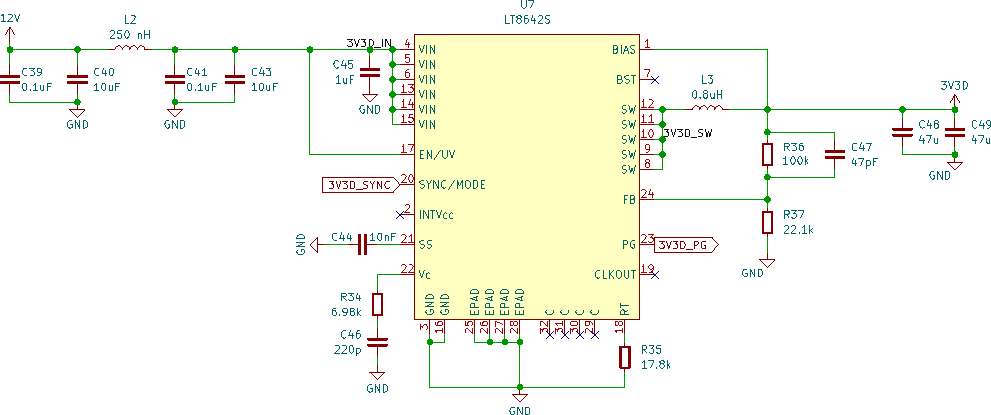
\includegraphics[width=0.8\linewidth]{sections/power/fig_3v3d.pdf}
  \caption{Digital \SI{3.3}{\volt} Step-Down DC-DC Converter Circuit}
  \label{fig:power_3v3d}
\end{figure}



\subsection{Analog \SI{5.5}{\volt} (5V5A)}

Analog \SI{5.5}{\volt} (5V5A) powers low noise analog LDO that supply analog front end and ADC. We selected the Analog Devices LT8624S synchronous step-down DC-DC converter that features:
\begin{itemize}
    \item Ultralow \SI{4}{\nano\volt/\sqrtunit{\hertz}} RMS noise (Silent Switcher 3 architecture).
    \item High efficiency.
    \item Ultra fast transient response: \SI{1}{\micro\second}.
    \item Up to \SI{4}{\ampere} continuous output current.
    \item External compensation.
\end{itemize}

The LT8624S is configured to operate at \SI{2}{\mega\hertz} (see \autoref{fig:power_5v5a}). A Coilcraft XGL1313-222 shielded inductor (\SI{2.2}{\micro\henry}, \SI{1.4}{\milli\ohm} DCR) minimizes losses. Upstream of the converter input, a $\pi$ LC filter suppresses input noise. Enable (\texttt{5V5A\_EN}), Power-Good output (\texttt{5V5A\_PG}) and the SYNC pin (\texttt{5V5A\_SYNC}) are connected to the Zynq SoC for enabling, voltage monitoring and clock synchronization. See LTSpice and LTPoweCAD simulation files for transient and frequency compensation design.

\begin{figure}[ht]
  \centering
  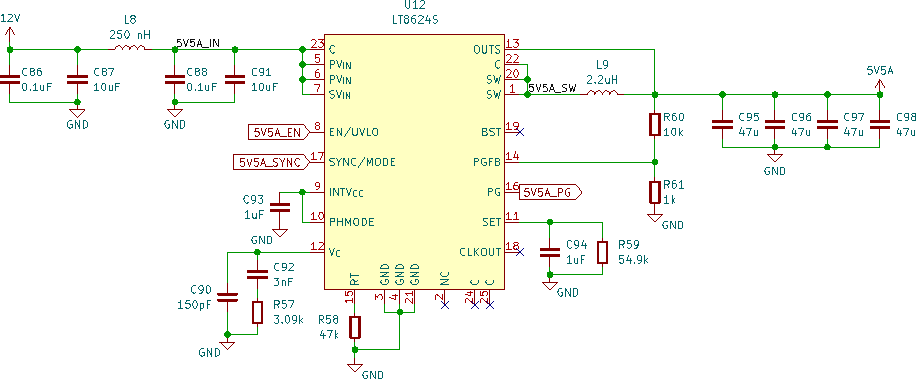
\includegraphics[width=0.8\linewidth]{sections/power/fig_5v5a.pdf}
  \caption{Analog \SI{5.5}{\volt} Step-Down DC-DC Converter Circuit}
  \label{fig:power_5v5a}
\end{figure}

\subsection{Analog \SI{15.5}{\volt} (+15V5A)}

The Analog \SI{15.5}{\volt} (+15V5A) DC-DC converter powers the low-noise Analog \SI{15}{\volt} LDO (15VA). We chose the Analog Devices LT8350S synchronous buck-boost converter that features:

\begin{itemize}
    \item 4-switch single inductor architecture.
    \item Low EMI (Silent Switcher 2 architecture).
    \item Up to 95\% efficiency at \SI{2}{\mega\hertz}.
    \item $\pm$1.5\% output voltage regulation.
    \item External compensation.
\end{itemize}

The LT8350S is configured to operate at \SI{2}{\mega\hertz} (see \autoref{fig:power_15v5a}). A Coilcraft XGL1313-222 shielded inductor (\SI{2.2}{\micro\henry}, \SI{1.4}{\milli\ohm} DCR) minimizes losses. Upstream of the converter input, a $\pi$ LC filter suppresses input noise. Enable (\texttt{15V5A\_EN}), Power-Good output (\texttt{15V5A\_PG}) and the SYNC pin (\texttt{15V5A\_SYNC}) are connected to the Zynq SoC for enabling, voltage monitoring and clock synchronization. See LTSpice and LTPoweCAD simulation files for transient and frequency compensation design.

\begin{figure}[ht]
  \centering
  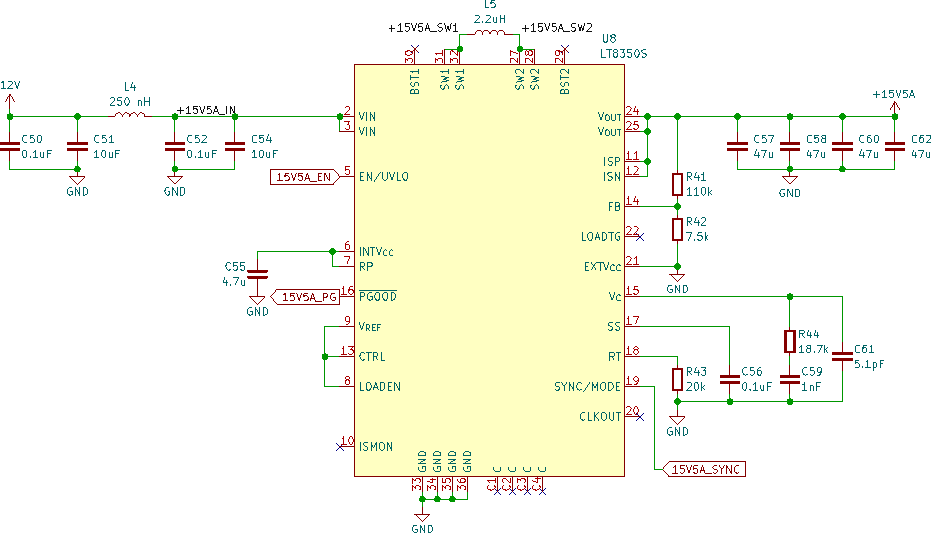
\includegraphics[width=0.8\linewidth]{sections/power/fig_15v5a.pdf}
  \caption{Analog \SI{15.5}{\volt} Buck-Boost DC-DC Converter Circuit}
  \label{fig:power_15v5a}
\end{figure}

\subsection{Analog \SI{-15.5}{\volt} (-15V5A)}

Analog \SI{-15.5}{\volt} (-15V5A) DC-DC converter powers the low-noise \SI{-15}{\volt} LDO (-15VA). We choose the Analog Devices LT3579 synchronous boost-inverting DC-DC converter that features:
\begin{itemize}
    \item \SI{6}{\ampere}, \SI{42}{\volt} combined power switch.
    \item Output short circuit protection.
    \item Configurable as inverting converter.
    \item External compensation.
\end{itemize}

The LT3579 is configured to operate at \SI{2}{\mega\hertz} (see \autoref{fig:power_n15v5a}). An Eaton DRQ-125-3R3-R coupled inductor (\SI{3.3}{\micro\henry}, \SI{6.3}{\milli\ohm} DCR) minimizes losses. Upstream of the converter input, a $\pi$ LC filter suppresses input noise. Enable (\texttt{-15V5A\_EN}), Power-Good output (\texttt{-15V5A\_PG}) and the SYNC pin (\texttt{-15V5A\_SYNC}) are connected to the Zynq SoC for enabling, voltage monitoring and clock synchronization. See LTSpice for transient design.

\begin{figure}[ht]
  \centering
  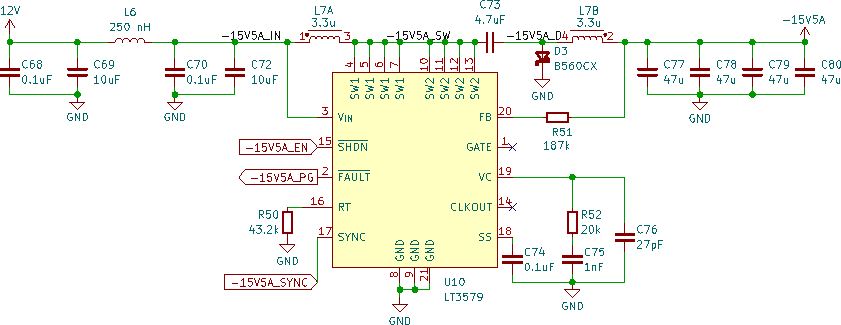
\includegraphics[width=0.8\linewidth]{sections/power/fig_n15v5a.pdf}
  \caption{Analog \SI{-15.5}{\volt} Inverting DC-DC Converter Circuit}
  \label{fig:power_n15v5a}
\end{figure}

\subsection{Linear Regulators}

The board requires multiple low-noise linear regulators to generate the analog and digital rails from the protected input supply. The following voltages are provided:
\begin{itemize}
    \item Analog Supplies: \SI{15}{\volt} (15VA), \SI{-15}{\volt} (-15VA), \SI{5}{\volt} (5VA), \SI{4.2}{\volt} (4V2A) and \SI{2.5}{\volt} (2V5A) for the analog front-end, ADCs and any external circuitry.
    \item Digital Supplies: \SI{2.5}{\volt} (2V5D) for the ADC LVDS and the Zynq SoC LVDS I/O bank.
\end{itemize}

All rails are generated by Analog Devices LT3042 (15VA), LT3093 (-15VA) and LT3045 (5VA, 4V2A, 2V5A and 2V5D ) ultra-low noise LDOs. These regulators offers:
\begin{itemize}
    \item Extremely low output noise: \SI{0.8}{\micro\volt} RMS (\SI{10}{\hertz} to \SI{100}{\kilo\hertz}) and \SI{2}{\nano\volt/\sqrtunit{\hertz}} at \SI{10}{\kilo\hertz}.
    \item Ultrahigh PSRR: \SI{73}{\decibel} (LT3093), \SI{76}{\decibel} (LT3045) and \SI{79}{\decibel} (LT3042)  at \SI{1}{\mega\hertz}.
    \item \SI{500}{\milli\ampere} (LT3045) and \SI{200}{\milli\ampere} (LT3093 and LT3042) output current.
\end{itemize}

\autoref{fig:power_5va} shows the schematic of the analog \SI{5}{\volt} regulator. Aside from the different resistor values used for setting the output voltage and the power-good feedback network, all LDO circuits follow the same layout. Each device's Enable (\texttt{EN}) and Power-Good (\texttt{PG}) pins are connected back to the Zynq SoC for centralized sequencing and fault monitoring.

\begin{figure}[ht]
  \centering
  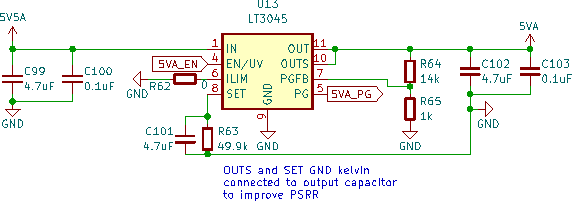
\includegraphics[width=0.8\linewidth]{sections/power/fig_5va.pdf}
  \caption{Analog \SI{5}{\volt} LDO Circuit}
  \label{fig:power_5va}
\end{figure}
\section{Clock Generator}

The clock generator derives an ultra-low-jitter timing reference from the single-ended \SI{10}{\mega\hertz} backplane synchronization signal (\texttt{CLOCK\_SYNC}). We use the Skyworks Si5342A-D jitter-attenuating clock multiplier, which provides:

\begin{itemize}
    \item Ultralow \SI{90}{\femto\second} RMS output jitter.
    \item Support for external crystals between \SI{25}{\mega\hertz} and \SI{54}{\mega\hertz}.
    \item SPI/I²C control interface.
    \item Zero-delay mode for minimal, deterministic input-to-output latency.
    \item Both single-ended and differential I/O.
\end{itemize}

The Si5342A-D “cleans” the backplane clock to produce a low-jitter reference. The Zynq SoC then employs this cleaned clock for its sequencer timing and to drive the DC-DC converters, reducing their switching noise and improving overall power-rail integrity.

In our design (see \autoref{fig:clock_gen}), a Kyocera AVX \SI{48}{\mega\hertz} $\pm$ 10ppm crystal provides the Si5342A-D's reference frequency. The device is configured in zero-delay mode to guarantee a fixed, repeatable phase relationship between \texttt{CLOCK\_SYNC} and the output clock to Zynq SoC. Configuration and status monitoring are handled over I²C via the Zynq SoC's. Finally, the Si5342A-D's differential \SI{2.5}{\volt} LVDS output is routed directly into one of the Zynq SoC's MRCC (Multi-Region Clock-Capable) input.

\begin{figure}[ht]
  \centering
  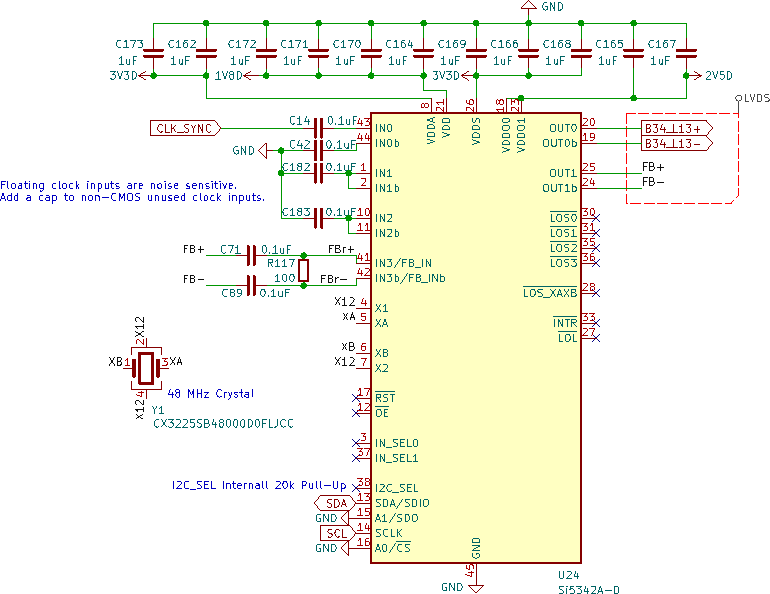
\includegraphics[width=0.8\linewidth]{sections/clock_gen/fig_clock_gen.pdf}
  \caption{Si5342A-D Clock Generator Jitter Attenuator Circuit}
  \label{fig:clock_gen}
\end{figure}
\section{Analog Front-End and ADC}

The analog front-end of the 4-channel ADC module is organized as two-stage chain that conditions each video input before digitalization. \autoref{fig:front_end_adc} illustrates the complete signal path for a single video channel. First, a low-noise instrumentation amplifier provides a well-defined return path, input impedance and gain for the input differential signal from detector. Second, a Fully Differential amplifier implements a low-pass filter and sets common-mode voltage for ADC. And finally, a high-speed SAR ADC samples the video signal and send data to Zynq SoC through \SI{2.5}{\volt} LVDS.

\begin{figure}[ht]
  \centering
  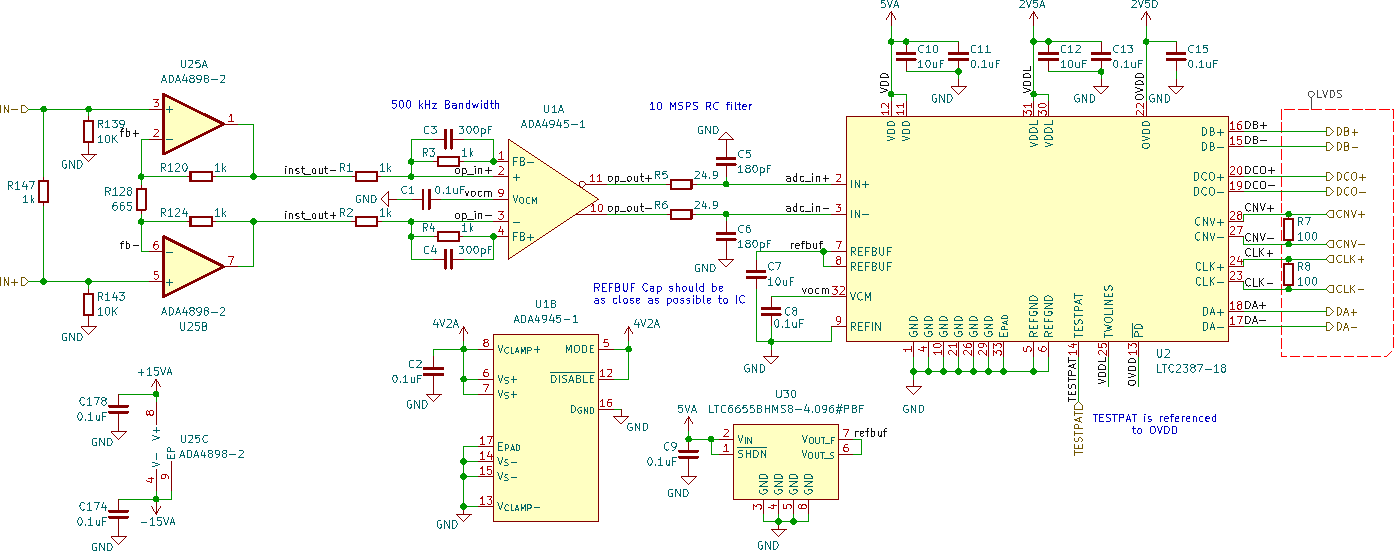
\includegraphics[width=1\linewidth]{sections/front_end_adc/fig_front_end_adc.pdf}
  \caption{Analog Front-End and ADC Circuit.}
  \label{fig:front_end_adc}
\end{figure}

Using Analog Devices Signal Chain Designer, the total noise refered to the input from \SI{0.1}{\hertz} to \SI{5}{\mega\hertz} is \SI{12.9}{\micro\volt_{rms}}, where:

\begin{itemize}
    \item Instrumentation amplifier: \SI{2.94}{\micro\volt_{rms}}.
    \item Fully differential amplififer: \SI{3.52}{\micro\volt_{rms}}.
    \item ADC: \SI{12}{\micro\volt_{rms}}.
\end{itemize}

Referred to front-end input:
\begin{itemize}
  \item Input signal swing: $v_\text{in}^\text{max} = 8.192/4 = \SI{2.05}{\volt}$ (DC gain of \SI{4}{\volt/\volt} and ADC input range of \SI{8.192}{\volt}).
  \item AC max signal: $v_\text{in,AC}^\text{max} = v_\text{in}^\text{max}/2/\sqrt{2} = \SI{723}{\milli\volt_{rms}}$.
  \item Signal chain noise: $n_\text{in} = \SI{12.9}{\micro\volt_{rms}}$.
  \item The Signal-to-Noise ratio (SNR): $20\log_{10}(v_\text{in,AC}^\text{max}/n_\text{in}) = \SI{94.99}{\decibel}$.
  \item Effective-Number-of-Bits (ENOB) without distortion: $(\text{SNR} - 1.76)/6.02 = \SI{15.49}{\bit}$.
\end{itemize}

\subsection{Instrumentation Amplifier}

\autoref{fig:inst_amp} shows the two opamp instrumentation amplifier equivalent circuit. Resistor $R_1=\SI{1}{\kilo\ohm}$ and $R_2=\SI{10}{\kilo\ohm}$ define input impedance, common mode path and return path for video input. Output common-mode voltage is maintaned and differential gain $G_1$ is set by $R_3 = \SI{665}{\ohm}$ and $R_4 = \SI{1}{\kilo\ohm}$ $\pm$\SI{0.1}{\percent} as:

\begin{equation}
    G_1 \equiv \frac{v_\text{out}}{v_\text{in}} =\frac{{v_\text{out}^+-v_\text{out}^-}}{v_\text{in}^+-v_\text{in}^-}= 1+\frac{2R_4}{R_3} \approx \SI{4}{\volt/\volt}
\end{equation}

\begin{figure}[ht]
  \centering
  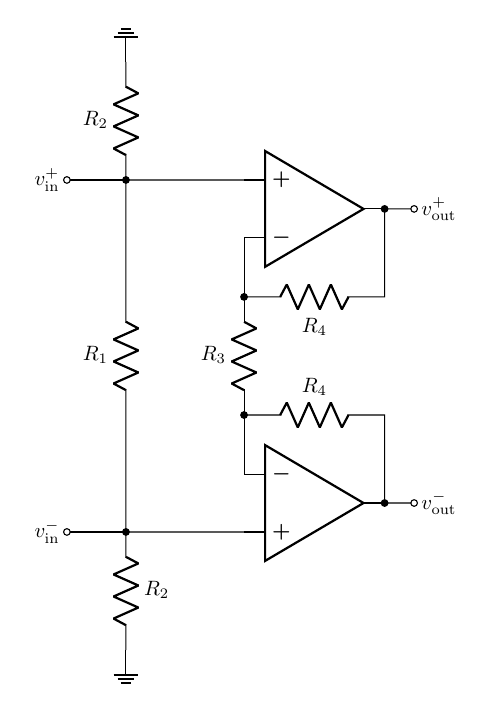
\begin{tikzpicture}[scale=0.75, transform shape]
    
    \draw (0,0) node[circ]{} coordinate(R3bot) to[R, l=$R_3$] ++(0,2) node[circ]{} coordinate (R3top);

    \draw (R3top) -- ++(0,1) node[op amp, yscale=-1, anchor=-] (A1){};
    \draw (R3bot) -- ++(0,-1) node[op amp, yscale=1, anchor=-] (A2){};

    \draw (A1.+) to[short,-*] ++(-2,0) coordinate (R1top);
    \draw (A2.+) to[short,-*] ++(-2,0) coordinate (R1bot);

    \draw (R1top) to[R, l=$R_2$] ++(0, 2) node[ground, yscale = -1]{};
    \draw (R1bot) to[R, l=$R_2$] ++(0, -2) node[ground]{};
    \draw (R1top) to[R, l_=$R_1$] (R1bot);

    \draw (R1top) -- ++(-1,0) node[ocirc]{} node[left]{$v_\text{in}^+$};
    \draw (R1bot) -- ++(-1,0) node[ocirc]{} node[left]{$v_\text{in}^-$};

    \coordinate (aux1) at (R3top -| A1.out);
    \coordinate (aux2) at (R3bot -| A2.out);

    \draw (R3top) to[R, l_=$R_4$] (aux1) -- (A1.out) node[circ]{} -- ++(0.5,0) node[ocirc]{} node[right]{$v_\text{out}^+$};
    \draw (R3bot) to[R, l^=$R_4$] (aux2) -- (A2.out) node[circ]{} -- ++(0.5,0) node[ocirc]{} node[right]{$v_\text{out}^-$};

\end{tikzpicture}
  \caption{Instrumentation Amplifier Equivalent Circuit.}
  \label{fig:inst_amp}
\end{figure}

For instrumentation amplifier we selected the Analog Devices ADA4898-2 dual operational amplifier that features:
\begin{itemize}
    \item Ultralow voltage noise: \SI{0.9}{\nano\volt/\sqrtunit{\hertz}} and \SI{2.4}{\pico\ampere/\sqrtunit{\hertz}} at \SI{1}{\kilo\hertz}.
    \item Ultralow distortion: \SI{-93}{\decibel c} at \SI{500}{\kilo\hertz}.
    \item High speed: \SI{65}{\mega\hertz} bandwidth at unity gain.
    \item Unity gain stable.
    \item Low input offset: \SI{160}{\micro\volt} maximum.
\end{itemize}

\subsection{Fully Differential Amplifier}

\autoref{fig:fda} shows the fully differential circuit equivalent circuit. Resistors $R_1=R_2=\SI{1}{\kilo\ohm}$ $\pm$ \SI{0.1}{\percent} define input impedance and differential gain. Output common-mode voltage is set externally by ADC to \SI{2.048}{\volt} and differential gain $G_2$ is set as:

\begin{equation}
    G_2 \equiv \frac{v_\text{out}}{v_\text{in}} =\frac{{v_\text{out}^+-v_\text{out}^-}}{v_\text{in}^+-v_\text{in}^-}= \frac{R_2}{R_1} = \SI{1}{\volt/\volt}
\end{equation}

The bandwidth BW is defined by $R_2$ and $C_1=\SI{300}{\pico\farad}$ for \SI{1}{\mega SPS} as:

\begin{equation}
    \text{BW} = \frac{1}{2\pi R_2 C_1} \approx \SI{530}{\kilo\hertz}
\end{equation}

\begin{figure}[ht]
  \centering
  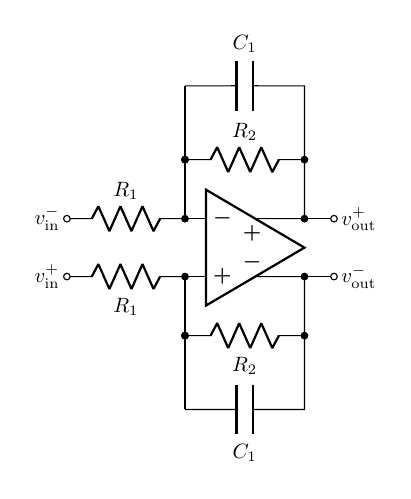
\begin{tikzpicture}[scale=0.75, transform shape]
    
    \draw (0,0) node[fd op amp] (opamp){};

    \draw (opamp.-) node[circ]{} -- ++(0,1) coordinate(opintop) node[circ]{};
    \draw (opamp.+) node[circ]{} -- ++(0,-1) coordinate(opinbot) node[circ]{};

    \draw (opamp.-) to[R, l_=$R_1$] ++(-2,0) node[ocirc]{} node[left]{$v_\text{in}^-$};
    \draw (opamp.+) to[R, l=$R_1$] ++(-2,0) node[ocirc]{} node[left]{$v_\text{in}^+$};

    \draw (opintop) to[R, l=$R_2$] (opintop -| opamp.out +) node[circ]{} -- (opamp.out +) node[circ]{};
    \draw (opinbot) to[R, l_=$R_2$] (opinbot -| opamp.out -) node[circ]{} -- (opamp.out -) node[circ]{};

    \draw (opintop) node[circ]{} -- ++(0,1.25) coordinate(rtop);
    \draw (opinbot) node[circ]{} -- ++(0,-1.25) coordinate(rbot);
    
    \draw (rtop) to[C, l=$C_1$] (rtop -| opamp.out +) -- (opintop -| opamp.out +);
    \draw (rbot) to[C, l_=$C_1$] (rbot -| opamp.out -) -- (opinbot -| opamp.out -);

    \draw (opamp.out +) -- ++(0.5,0) node[ocirc]{} node[right]{$v_\text{out}^+$};
    \draw (opamp.out -) -- ++(0.5,0) node[ocirc]{} node[right]{$v_\text{out}^-$};


\end{tikzpicture}
  \caption{Fully Differential Amplifier Equivalent Circuit.}
  \label{fig:fda}
\end{figure}

As fully differential amplifier we selected the Analog Devices ADA4945-1 in full-power mode that features:

\begin{itemize}
    \item Rail-to-rail output.
    \item \SI{4}{\milli\ampere} at full-power mode.
    \item \SI{145}{\mega\hertz} bandwidth at gain 1 at full-power mode.
    \item Low noise: \SI{2}{\nano\volt/\sqrtunit{\hertz}} at \SI{100}{\kilo\hertz}.
    \item \SI{115}{\micro\volt} maximum offset voltage.
\end{itemize}

\subsection{Analog-to-Digital Converter (ADC)}

\autoref{fig:filter} shows ADC input filter equivalent circuit. For an \SI{18}{\bit}, the error of a full scale range (FS) step in a single-pole $RC$ filter after acquisition time $t_\text{ACQ}$ is $\exp\left(-\frac{t_\text{ACQ}}{R_\text{filt}C_\text{filt}}\right)\text{FS}$ and a half LSB is approximately $2^{-19}\, \text{FS}$. Then we have

\begin{equation}
    \exp\left(-\frac{t_\text{ACQ}}{R_\text{filt}C_\text{filt}}\right)\text{FS} = 2^{-19}\,\text{FS} \Leftrightarrow C_\text{filt} = \frac{t_\text{ACQ}}{19R_\text{filt}\ln 2}
\end{equation}

\begin{figure}[ht]
  \centering
  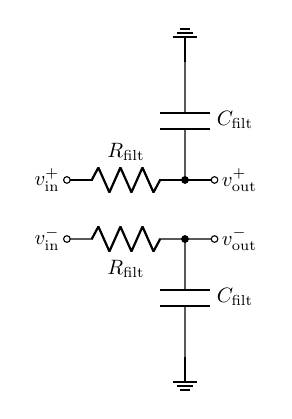
\begin{tikzpicture}[scale=0.75, transform shape]
    
    \draw (0,0) node[ocirc]{} node[left]{$v_\text{in}^+$} to[R, l=$R_\text{filt}$] ++(2,0) node[circ]{} coordinate(rtop){} -- ++(0.5, 0) node[ocirc]{} node[right]{{$v_\text{out}^+$}};

    \draw (0,-1) node[ocirc]{} node[left]{$v_\text{in}^-$} to[R, l_=$R_\text{filt}$] ++(2,0) node[circ]{} coordinate(rbot){} -- ++(0.5, 0) node[ocirc]{} node[right]{{$v_\text{out}^-$}};

    \draw (rtop) to[C, l_ = $C_\text{filt}$] ++(0,2) node[ground, yscale = -1]{};
    \draw (rbot) to[C, l = $C_\text{filt}$] ++(0,-2) node[ground, yscale = 1]{};

\end{tikzpicture}
  \caption{ADC Input filter Equivalent Circuit.}
  \label{fig:filter}
\end{figure}

We selected the Analog Devices LTC2387-18 \SI{18}{\bit} \SI{15}{\mega S P S} SAR ADC that features:

\begin{itemize}
    \item No pipeline delay, no cycle latency.
    \item \SI{95.7}{\decibel} SNR at \SI{1}{\mega\hertz}.
    \item \SI{102}{\decibel} SFDR at \SI{1}{\mega\hertz}.
    \item $\pm$\SI{3}{LSB} INL maximum.
    \item \SI{8.192}{\volt_{p-p}} differential input.
    \item \SI{2.5}{\volt} Serial LVDS interface.
\end{itemize}

For selected ADC we have $t_\text{ACQ} = 1/f_s -\SI{39}{\nano\second}$. For $f_s = \SI{10}{\mega SPS}$ sample rate and $R_\text{filt}=\SI{24.9}{\ohm}$ we get $C_\text{filt}\approx \SI{180}{\pico\farad}$.

To improve ADC reference voltage temperature drift,  reference out pin (\texttt{REFBUF}) is externally driven by Analog Devices LTC6655 \SI{4.096}{\volt} low drift voltage precision reference that features:

\begin{itemize}
  \item Low Noise: \SI{0.25}{ppm_{P-P}} (\SI{0.1}{\hertz} to \SI{10}{\hertz}).
  \item Low drift: \SI{2}{ppm/\degreeCelsius}.
  \item High accuracy: $\pm$\SI{0.025}{\percent} maximum.
  \item Long term drift: \SI{20}{ppm /\sqrtunit{\kilo\hour}}.
\end{itemize}
\section{Main Processor}

The main processor is in charge of generating the sequencer signals for reading the detector, configuring integrated circuits, monitoring interlocks, and communicating via Ethernet protocol. As main processor we selected the Trenz Electronic TE0720-04-62I33MA SoC-Module. \autoref{fig:soc} shows TE0720-04-62I33MA SoC-Module.

\begin{figure}[ht]
  \centering
  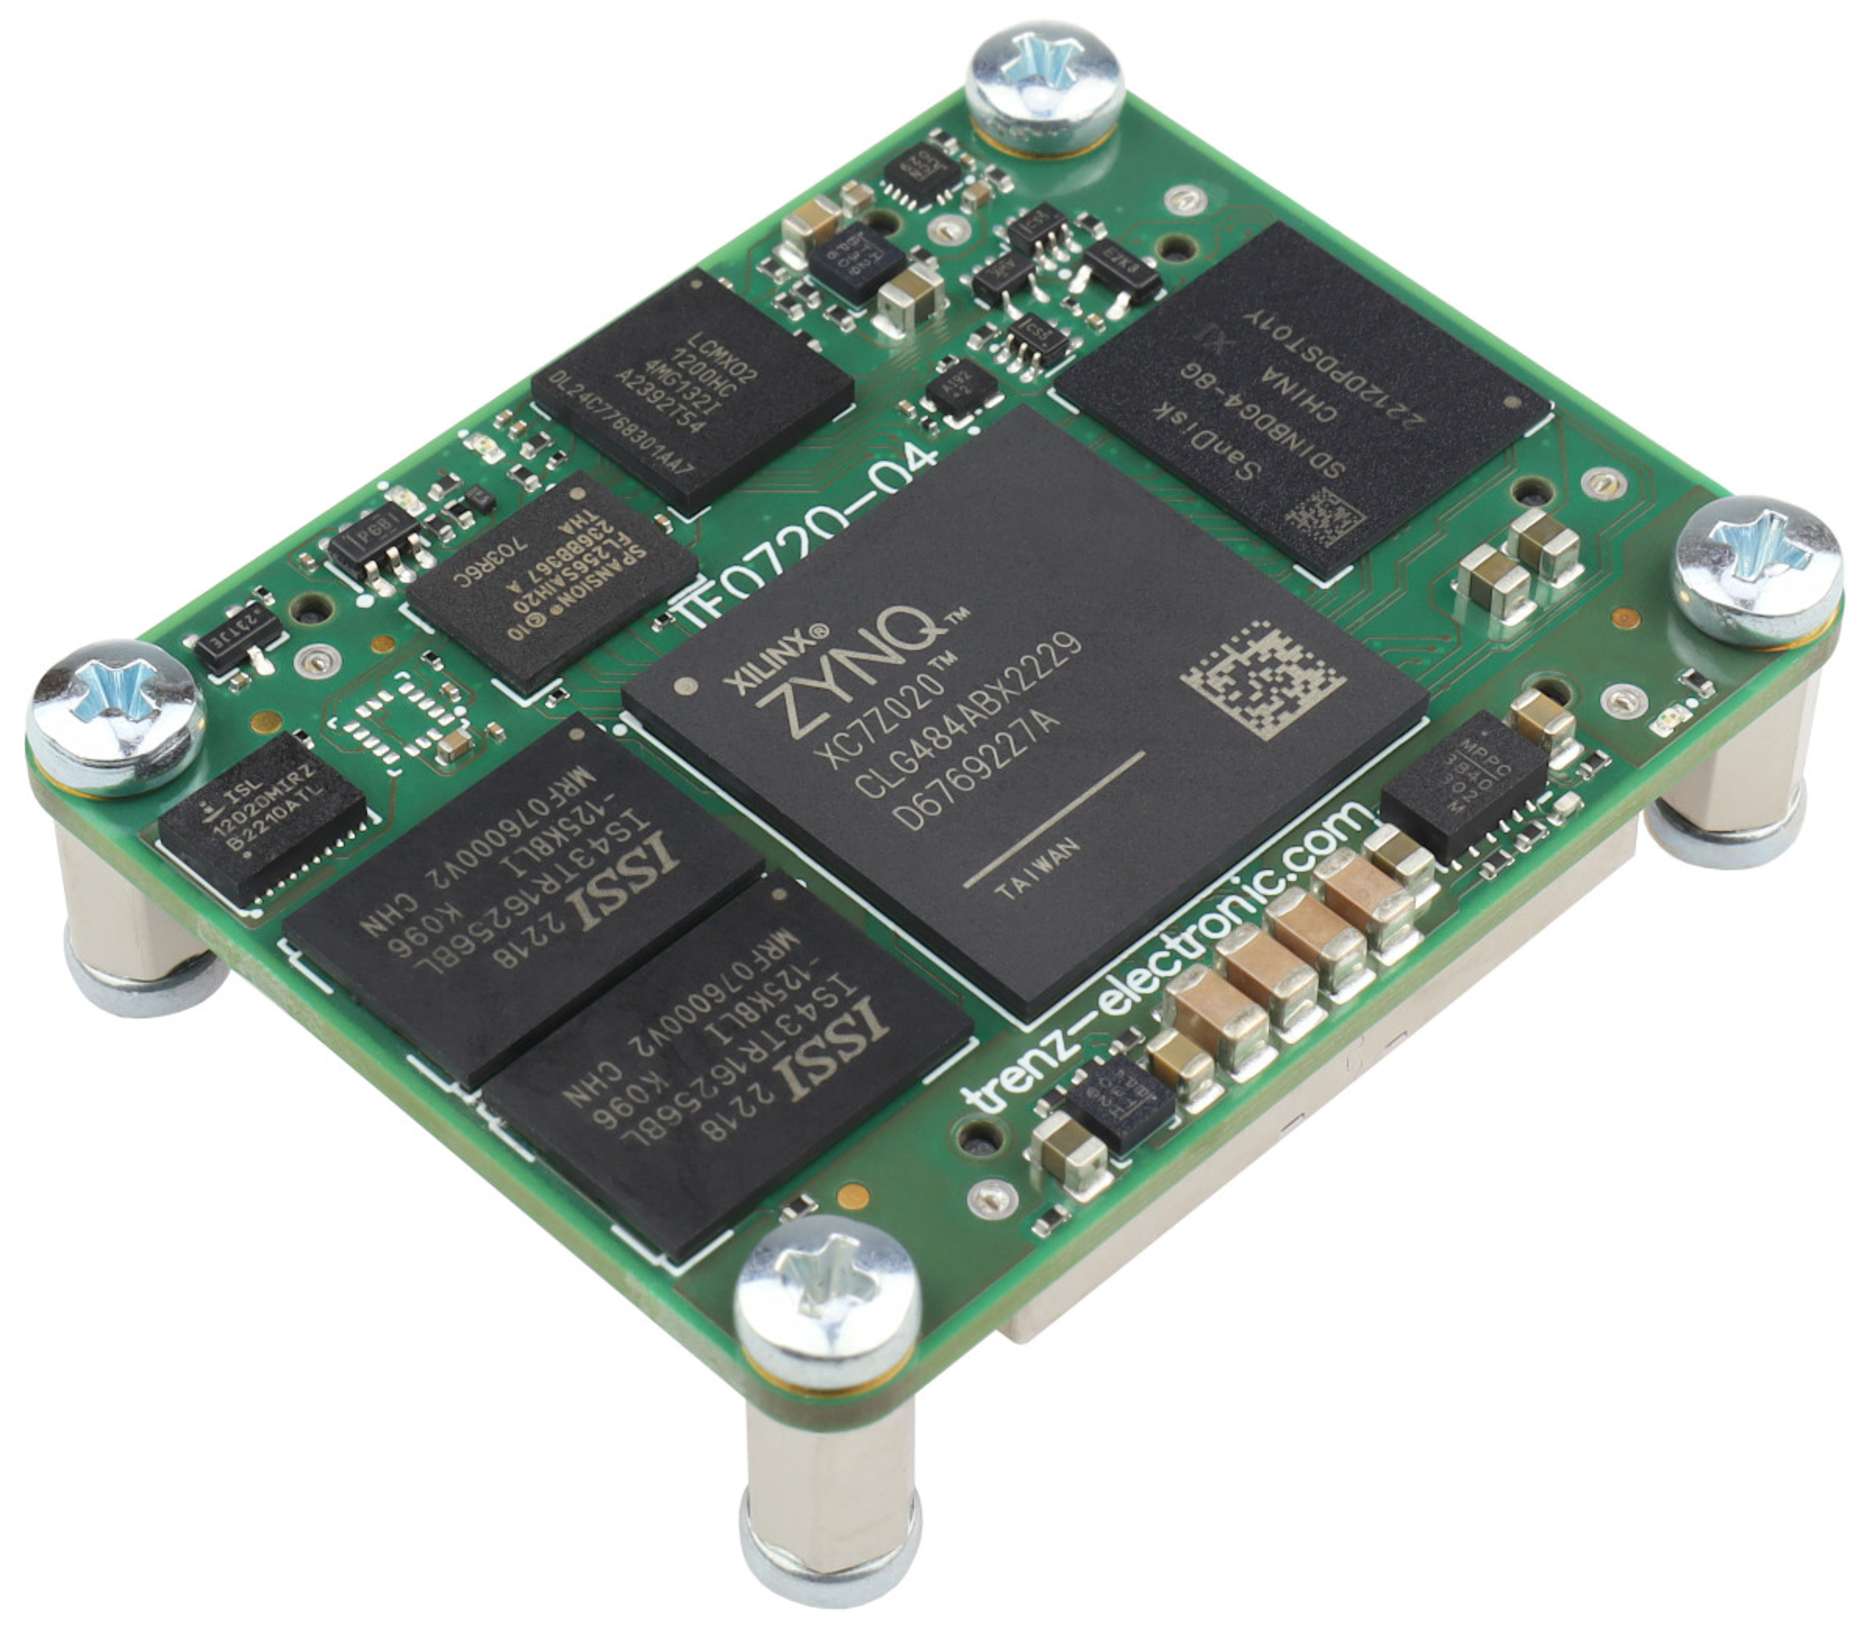
\includegraphics[width=0.6\linewidth]{sections/proc/soc.pdf}
  \caption{Trenz Electronic TE0720-04-62I33MA SoC-Module.}
  \label{fig:soc}
\end{figure}

Trenz Electronic TE0720-04-62I33MA SoC-Module features:

\begin{itemize}
    \item AMD Zynq™ XC7Z020-2CLG484I dual ARM® Cortex®-A9 MPCore™ with CoreSight™ System On Chip (SOC) IC Zynq®-7000 Artix™-7 FPGA, 85K Logic Cells 766MHz 484-CSPBGA (19x19).
    \item Rugged for high shock and vibration.
    \item 10/100/1000 tri-speed Gigabit Ethernet transceiver (PHY), SGMII accessible on a board-to-board connector.
    \item 1 GByte (32-bit) DDR3 SDRAM.
    \item 32 MByte QSPI Flash memory (for configuration and operation).
    \item 8 GByte e.MMC.
    \item Plug-on module with 2 x 100-pin and 1 x 60-pin Razor Beam High-Speed hermaphroditic Terminal/Socket Strips.
    \item 152 FPGA I/O's (75 LVDS pairs possible) and 14 MIOs available on board-to-board connectors.
    \item On-board high-efficiency DC-DC converters.
    \item Programmable through Free Vivado Standard Edition Suite.
\end{itemize}

Trenz Electronic TE0720-04-62I33MA SoC-Module is configured as: 

\begin{itemize}
    \item Low jitter clock input for sequencer and DC-DC synchronization from clock generator IC. 
    \item \SI{2.5}{\volt} external power supply for banks 13, 34 and 35. Bank 13 is not powered (unused).
    \item JTAG programming and UART communication through on board FTDI.
    \item \SI{3.3}{\volt} I2C communication through MIO pins for clock generator and EEPROM.
    \item \SI{2.5}{\volt} LVDS differential pair communication with ADC.
    \item Internal \SI{1.8}{\volt} is used for clock generator.
    \item Backplane communication through \SI{2.5}{\volt} to \SI{3.3}{\volt} voltage translator IC.
\end{itemize}
\section{Connectors}

\subsection{Backplane Connector}

Backplane connector serves as the primary interface for power, control, and monitoring systems. It brings in an external \SI{12}{\volt} power rail to feed board DC-DC converters and \SI{3.3}{\volt} digital I/O like synchronization and interlocks. 

Selected backplane connector is TE Connectivity 5747841-4 15-position D-Sub plug male pins connector. \autoref{tab:backplane} shows backplane connector pinout.

\begin{table}[ht]
  \centering
  \begin{tabular}{l c l c l}
    \toprule
    Pin name  & Pin no.     & Dir. & Level            & Description                                \\
    \midrule
    12VIN     & 7, 8, 15        & —    & \SI{12}{\volt}   & External power input                       \\[3pt]
    BPI0      & 1               & In   & \SI{3.3}{\volt}  & 10\,\si{\mega\hertz} external sync clock  \\
    BPI1      & 9               & In   & \SI{3.3}{\volt}  & Digital input                              \\
    BPI2      & 10              & In   & \SI{3.3}{\volt}  & Digital input                              \\
    BPI3      & 3               & In   & \SI{3.3}{\volt}  & Digital input                              \\[3pt]
    BPO0      & 4               & Out  & \SI{3.3}{\volt}  & Digital output                             \\
    BPO1      & 12              & Out  & \SI{3.3}{\volt}  & Digital output                             \\
    BPO2      & 13              & Out  & \SI{3.3}{\volt}  & Digital output                             \\
    BPO3      & 6               & Out  & \SI{3.3}{\volt}  & Digital output                             \\[3pt]
    GND       & 0, 2, 5, 11, 14 & —    & \SI{0}{\volt}    & Ground return                              \\
    \bottomrule
  \end{tabular}
  \caption{Backplane Connector Pinout}
  \label{tab:backplane}
\end{table}

Backplane connector digital I/O signals are translated from \SI{3.3}{\volt} to \SI{2.5}{\volt} and then connected to \SI{2.5}{\volt} Zynq SoC-Module bank 34. For voltage translation we selected a Texas Instrument SN74AXC8T245QPWRQ1 automotive \SI{8}{\bit} \SI{380}{\mega bps} dual-supply bus transceiver with ESD protection.

\subsection{USB-C Connector}

USB-C connector is used to program through JTAG and communicate through USART with Zynq SoC-Module using a USB converter.

Selected USB converter is FTDI FT2232HL USB Hi-Speed to Dual Channel Serial UART/FIFO/JTAG/SPI/I2C IC. FT2232HL \texttt{ADBUS} is used for JTAG and \texttt{BDBUS} us used for UART. UART \texttt{RXD} (Zynq to host) is connected to Zynq \texttt{MIO15} and \texttt{TXD} (host to Zynq) is connected to Zynq \texttt{MIO14}. 

\subsection{Gigabit Ethernet Connector}

Gigabit ethernet connector is RJ45 connector used for communication between Zynq SoC-Module Ethernet PHY and host for configuration, telemetry and video streaming.

Selected Gigabit ethernet connector is Taoglas TMJG4820GENL industrial grade RJ45 connector with integrated magnetics 1G Base-T that features EMI finger and short body. Internal LEDs are disabled. 

\subsection{Video Input Connector}

Video input connector contains 4 differential video input pairs and also provides $\pm$\SI{15}{\volt} analog input to power external pre-amplifiers.

Selected video input connector is TE Connectivity 5747841-4 15-position D-Sub plug male pins connector. \autoref{tab:video} shows video input connector pinout.

\begin{table}[ht]
  \centering
  \begin{tabular}{l c l c l}
    \toprule
    Pin name  & Pin no.     & Dir. & Level            & Description                                \\
    \midrule
    +15VA 	& 1   	& Out  	& \SI{15}{\volt}   	& Analog power output          	\\
    -15VA  	& 8 	& Out  	& \SI{-15}{\volt} 	& Analog power output  			\\[3pt]
	
	IN0+	& 10	& In	& $\pm$\SI{15}{\volt}					& Channel 0 Video Input +		\\
	IN0-	& 2	    & In	& $\pm$\SI{15}{\volt}					& Channel 0 Video Input -		\\
	IN1+	& 4	    & In	& $\pm$\SI{15}{\volt}					& Channel 1 Video Input +		\\
	IN1-	& 11	& In	& $\pm$\SI{15}{\volt}					& Channel 1 Video Input -		\\
	IN2+	& 13	& In	& $\pm$\SI{15}{\volt}					& Channel 2 Video Input +		\\
	IN2-	& 5	    & In	& $\pm$\SI{15}{\volt}					& Channel 2 Video Input -		\\
	IN3+	& 7	    & In	& $\pm$\SI{15}{\volt}					& Channel 3 Video Input +		\\
	IN3-	& 14	& In	& $\pm$\SI{15}{\volt}					& Channel 3 Video Input -		\\[3pt]
	
    GND    	& 3, 6, 9, 12, 15 & —    & \SI{0}{\volt}    & Ground return  		\\

    \bottomrule
  \end{tabular}
  \caption{Video Input Connector Pinout}
  \label{tab:video}
\end{table}
\section{Miscellaneous}

\subsection{EEPROM}

An EEPROM (Electrically Erasable Programmable Read-Only Memory) is used to store PCB board ID and model.

Selected EEPROM is Microchip 24LC16BT-I/OT \SI{16}{\kilo\bit} non-volatile I2C EEPROM. 

% Bibliography (if needed)
% \bibliographystyle{ieeetr}
% \bibliography{bib/references}

\end{document}
